\chapter{General Discussion}\thumbforchapter
\newpage

\section{The phylotypic stage}

\begin{shadequote}[c]{George Box}
All models are wrong, but some are useful.
\end{shadequote}

While historically, the phylotypic stage has predominantly been examined and described through qualitative methods, the 21\textsuperscript{st} century started a paradigm shift towards a more quantitative and data-driven approach to understanding this phenomenon\cite{Chan2021}. The first notable quantitative investigation into the phylotypic stage was done by Bininda-Emonds \textit{et al.}, where they calculated temporal conservation as the order in which morphological embryonic features appear in vertebrates\cite{OlafRP2003}. However, it wasn't until the early 2010s that the field truly embraced quantitative methodologies with the simultaneous publication of two groundbreaking studies in Nature\cite{Kalinka2010, DomazetLoso2010}. In these works, Domazet-Lošo \textit{et al.} investigated the average developmental age of transcripts in \textit{D. rerio} and \textit{D. melanogaster}, whilst at the same time, Kalinka \textit{et al.} explored the temporal transcriptome similarities across different \textit{Drosophila} species. These molecular studies opened a new line of research to the quantitative basis of the phylotypic stage. The quantitative support for the phylotypic stage appeared stronger and stronger with each new study. So strong, that we quickly forgot all the nonconforming studies.

The Transcriptome Age Index (TAI), as introduced by Domazet-Lošo \textit{et al.}, is a metric of the average evolutionary age of transcripts over time\cite{DomazetLoso2010}. Evolutionary age is determined as the number of taxonomic branches to which a gene can be traced back. The central idea of the TAI is that temporal changes in gene expression provide insights into the degree of conservation during development. However, a re-analysis conducted by Piasecka \textit{et al.} raised some critical points about the methodology\cite{Piasecka2013}. Their investigation revealed that the TAI is heavily influenced by a relatively small subset of genes due to major differences in transcript levels per gene (transcriptomic data is notoriously heteroscedastic). Log transforming the data, which is a standard processing step for this type of data, completely invalidates the results of the original study. One might expect such a dependency on data transformation to cast doubts on the method's reliability. Surprisingly, the opposite appears to be true. The original study introducing the TAI has been cited 88 times between 2010 and 2013, and 359 citations since Piasecka \textit{et al.}'s publication (covering the years 2014-2023). As it turns out, you can now analyze the data with and without transformation, and keep the results that reinforce your preferred hypothesis. A notable example of this is found in Wu \textit{et al.}'s study on Spiralian development\cite{Wu2019}. In their analysis of untransformed data for \textit{Crassostrea gigas}, \textit{Haliotis discus hannai}, and \textit{Perinereis aibuhitensis}, they claim to have found an inverse hourglass pattern. However, their supplementary data reveals a different pattern for \textit{Crassostrea gigas} after square root transformation, shifting from an inverse hourglass to a funnel shape. Remarkably, this crucial finding receives minimal attention in the study, with the authors merely stating that at least the transformed data does not show an hourglass-like pattern. Moreover, the transformed TAI of the other two species are not even shown. It's also noteworthy that the inverse hourglass pattern of \textit{Perinereis aibuhitensis} of untransformed data can be attributed to random noise. Where this study should be taken with a grain of salt, it has sparked a discussion among three influential evolutionary-developmental biologists - Pavel Tomanczak, Denis Duboule, and Andreas Hejnol - on Twitter, about the universality of the hourglass model. It's worth mentioning that Andreas Hejnol has authored two critical reviews of previous studies that asserted the universality of the phylotypic stage\cite{Dunn2018,hejnol2016}.

The work of Barbara Piasecka, where she showed that the pattern of the TAI is caused by a subset of all genes was led by Marc Robinson-Rechavi. The main work of this study was not about the TAI, but about using a multitude of different metrics to estimate temporal evolutionary conservation. Their conclusion is that different metrics give different results. This is important, as it raises questions about the inherent complexity of measuring (temporal) conservation and underscores the potential influence of the chosen methodology. Marc Robinson-Rechavi's later career appears to have diverged from his earlier findings. He has made assertive claims concerning the ortholog conjecture\cite{KryuchkovaMostacci2016} and the hourglass model of conservation\cite{Liu2020,Liu2021,marletaz2018}. A re-analysis by Casey Dunn \textit{et al.} identified methodological issues with their analysis of the ortholog conjecture\cite{Dunn2018}, and in chapter \textbf{X} I discuss in detail the methodological problems of two of his studies related to the hourglass model.

In 2003, Bininda-Emonds \textit{et al.} conducted a quantitative study of the phylotypic stage, which was revisited by Gerardo A. Cordero \textit{et al.} seventeen years later\cite{OlafRP2003, Cordero2020}. Both studies were about the quantitative temporal analysis of morphological characteristics. To the best of my knowledge, these are the only quantitative analyses of morphological characteristics with respect to the phylotypic stage. Bininda-Emonds et al.'s initial findings revealed an unexpected inverse hourglass pattern in morphological rankings, a discovery that challenged existing assumptions. However, the later study of Cordero \textit{et al.} shows precisely the opposite - an hourglass pattern. Surprisingly, Cordero \textit{et al.} only comment that the difference between these two studies \textit{could} be caused by a difference in morphological characteristics, methodology, and species used, without any further analysis of the differences. The main analysis of Bininda-Emonds \textit{et al.} is a mean-variance plot, something that takes 5 minutes to generate, and it is truly puzzling why Cordero \textit{et al.} did not repeat this analysis.

In 2016, Levin \textit{et al.} introduced the transcriptomic inverse hourglass model as a potential method for distinguishing between different phyla\cite{Levin2016}. However, this study has been rightfully criticized by Casey Dunn and Andreas Hejnol for its lack of a within-phylum control\cite{hejnol2016} and incorrect statistical methods\cite{Dunn2018}. Given the ambitious claim of a "universal" phylotypic stage characterized by high similarity within phyla but low similarity between phyla, it is somewhat perplexing that these criticisms have not yet been addressed by Levin \textit{et al}. What makes the situation even more perplexing is that another group of evolutionary developmental biologists compared the embryonic development of deuterostomes and the chordate amphioxus - a between-phyla comparison. Astonishingly, they uncovered an hourglass-like pattern\cite{PerezPosada2022}, directly contradicting Levin \textit{et al.}'s inverse hourglass model, but fail to comment on this. In Chapter XXX, I present evidence that the transcriptomic inverse hourglass is a statistical artifact resulting from normalization rather than an accurate representation of temporal conservation. 
\begin{figure}[H]
    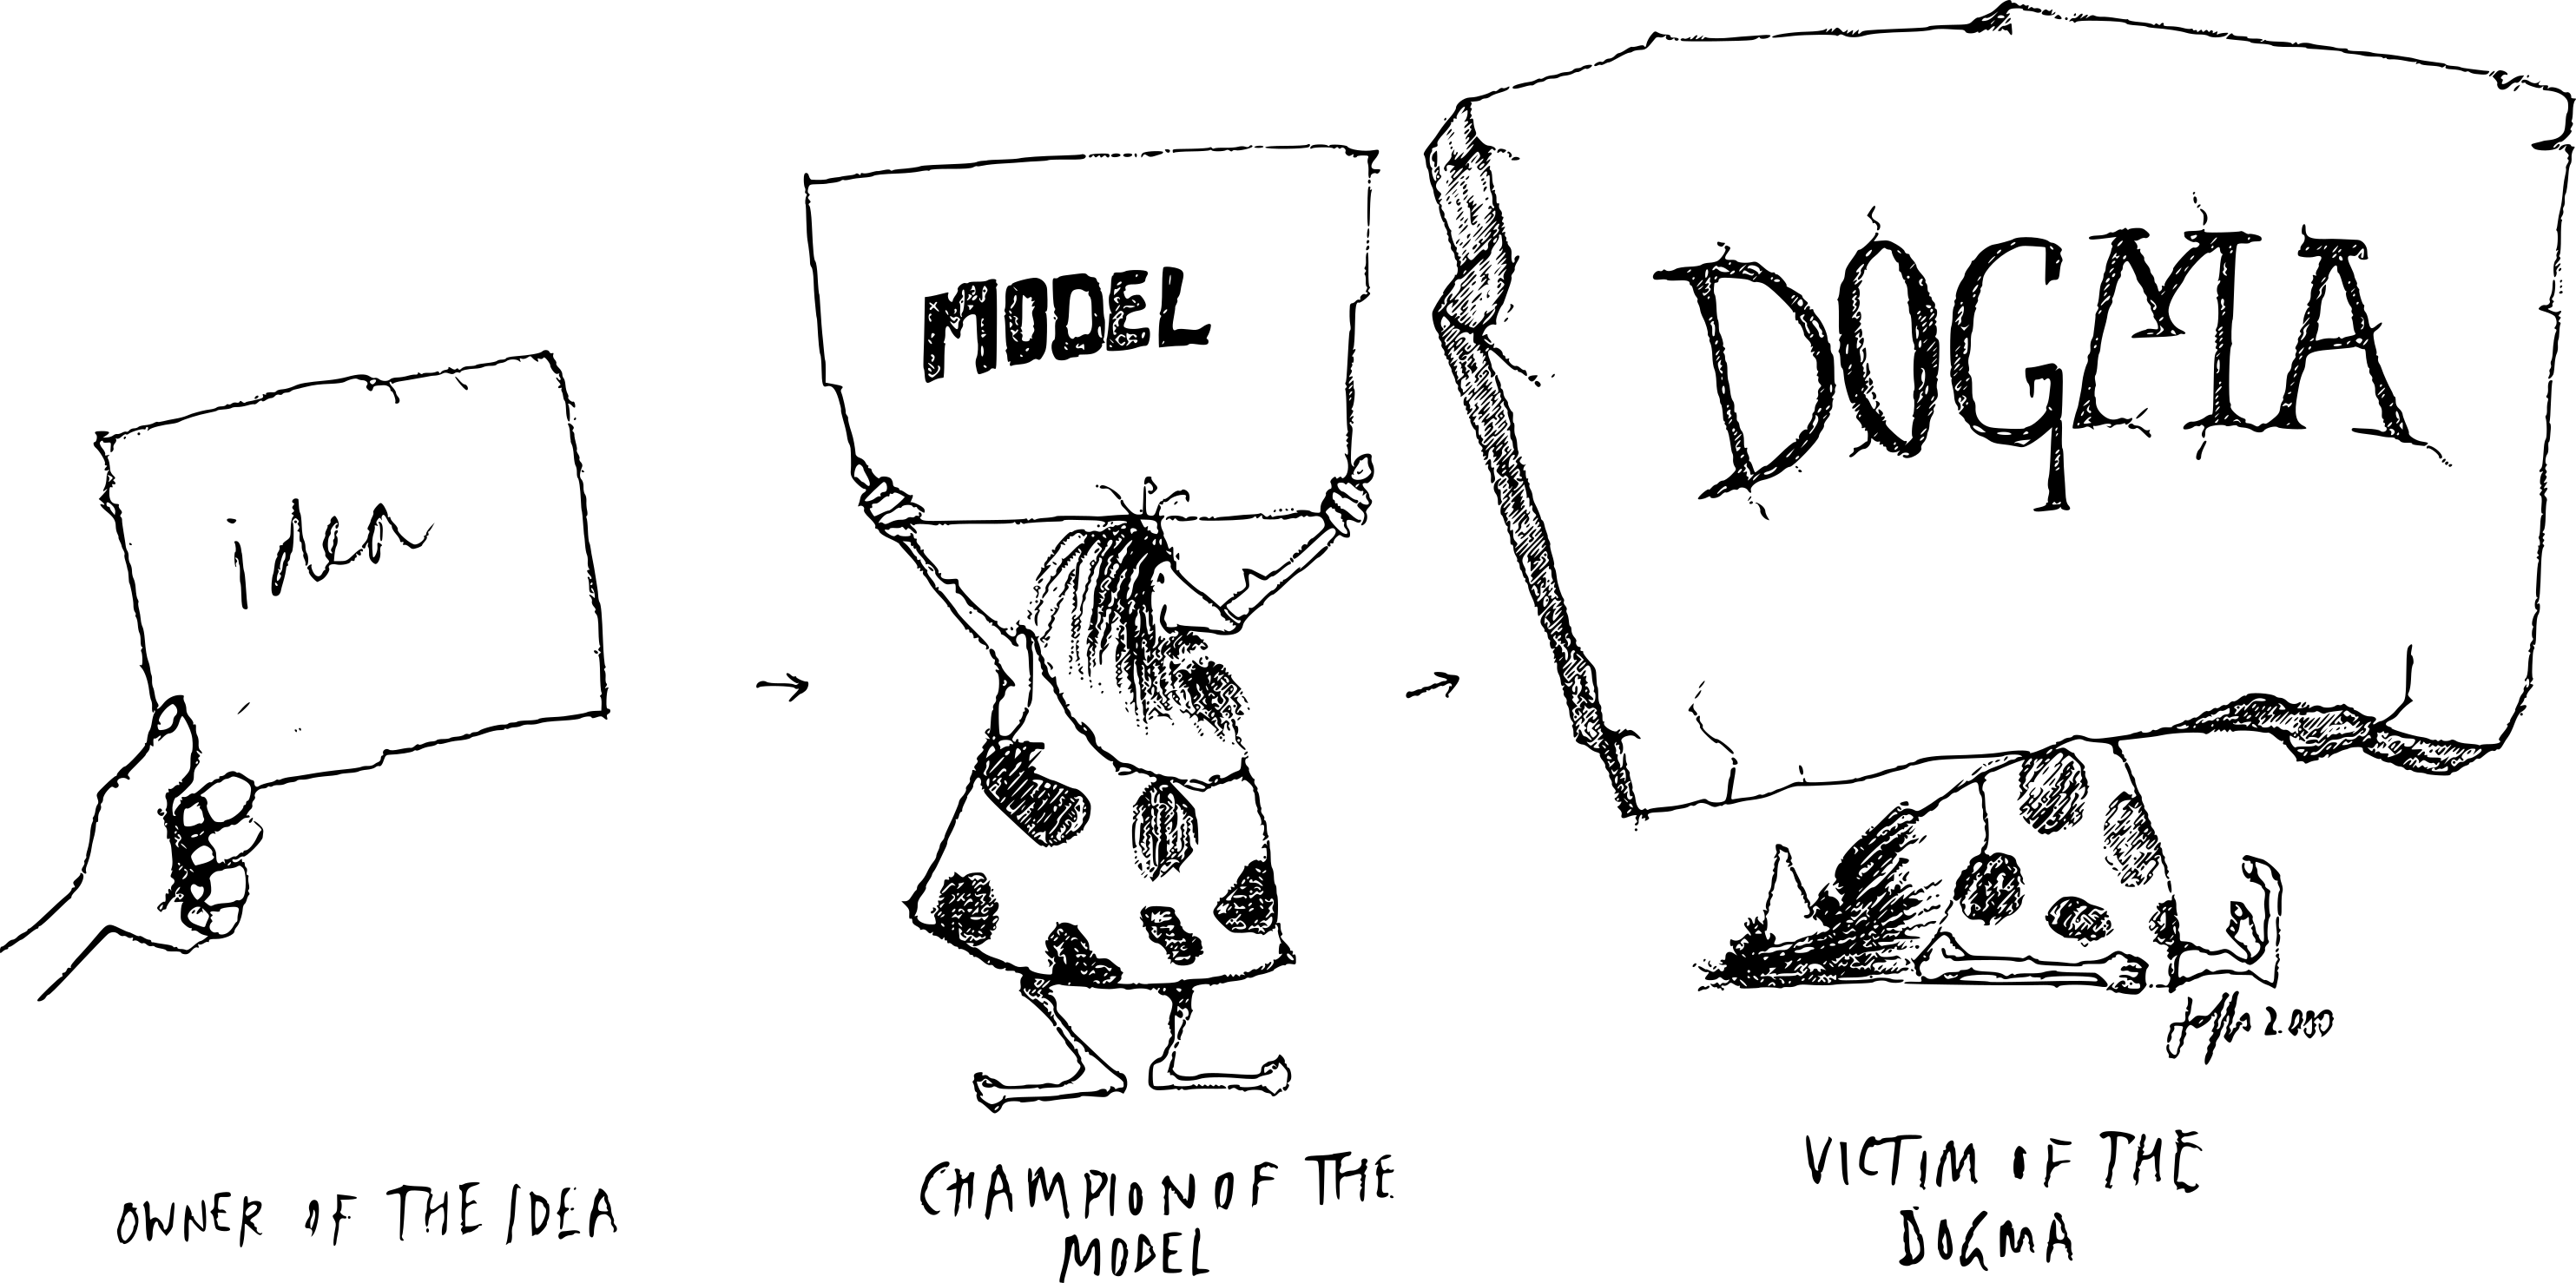
\includegraphics[width=\linewidth]{ch.discussion/imgs/dogma.png}
    \caption{\textbf{The phylotypic stage as a dogma} \cite{Caveman2000}.}
    \label{fig:dogma}
\end{figure}

Yoav Mayshar \textit{et al.} studied the phylotypic stage and the hourglass model from a single-cell point of view\cite{Mayshar2023}. Their research involved a comparative analysis of cell type proportions during the development of rabbit and mouse embryos. However, in Chapter X, I show that both the rabbit time series and the mouse time series exhibit discontinuous patterns. These discontinuities significantly influence the temporal correlations between the two species. This discontinuous pattern in cell-type proportions could be interpreted as indicative of a mid-developmental transition, resembling an inverse hourglass-like pattern. What raises questions is Mayshar \textit{et al.}'s interpretation of this data. They perceive the pattern as confirming the traditional hourglass model. This leads to the question of why such a fundamental problem of their analysis was not detected during the peer review process, especially considering that the study was published in Cell, one of the most prestigious scientific journals. When I asked Y. Mayshar on Twitter if their results perhaps represent an inverse hourglass, he commented with \say{this basically shows convergence of frequencies of cell states at \textasciitilde e7.5-e8, preceding what would be normally considered as the phylotypic stage, though this is pretty vaguely defined...}. Pretty vague indeed Yoav.

There appears to be a concerning lack of genuine effort to understand or engage with one another's work within the field. Many studies, it seems, are riddled with glaring methodological issues that often go unaddressed, as long as they align with our prior beliefs. In chapters X AND Y I show and discuss a series of newly discovered problems with comparative approaches. I fear that highlighting these problems won't actually matter, as people will continue to believe their pet theories, and there will always be some methodology that in a way affirms it. For instance, during the early stages of my PhD, I had a meeting with Ozren Bogdanovic, one of the authors of the papers that does a transcriptomic comparisons between \textit{D. rerio} and \textit{X. tropicalis}. He is a staunch believer of the hourglass model, and even has a tattoo of it! I shared some of my preliminary findings with him, which pointed to the inverse hourglass being an artifact of normalization. I also expressed my concerns regarding the methodology employed in their analysis. Surprisingly, he brushed off my concerns, stating that he was not directly involved in that particular analysis and thus saw no need to discuss its potential issues. To this day, I remain perplexed as to why the identity of the analyst should bear any significance for the validity or relevance of the analysis. Similarly, a colleague in my department once commented that despite my work showing that virtually all quantitative methodologies used in our field are flawed, the undeniable fact remains that the phylotypic stage does, in fact, exist.

Based on my own re-analyses, it appears most methodologies actually support the null model. The null model for evolutionary embryonic development would be that there is no specific stage of higher or lower temporal conservation. 
\begin{itemize}
    \item The hourglass-like pattern between zebrafish and frogs based on transcriptomic correlations can be explained by within-species correlations alone.
    \item The pattern of cell type proportion similarity between rabbits and mice, which is wrongfully called an hourglass, can be explained by discontinuous temporal sampling.
    \item Both the transcriptomic between-phyla inverse hourglass pattern and the morphological within-phylum inverse hourglass pattern are fully reproduced by simulated data with no specific temporal conservation.
    \item Only the \textit{Drosophila} enhancer conservation re-analysis results in a stage of maximum similarity, albeit at a different point than the original authors find. Moreover, I simply do not agree with the methodological approach of this analysis.
\end{itemize}
Altogether, I have found little evidence to reject the null hypothesis of constant temporal conservation.

Furthermore, there is no consensus about what is actually expected to be conserved. The original observation that vertebrate embryos, perhaps, look more like each other at certain points in development than at other times, says nothing about the molecular basis for this. It has been quantitatively studied on the basis of embryonic lethality\cite{Uchida2018}, morphology\cite{OlafRP2003,Cordero2020}, DNA sequence conservation\cite{Piasecka2013,Quint2012,Liu2021} and activation order\cite{Uesaka2019}, cell type proportion\cite{Mayshar2023}, and whole-transcriptome similarity\cite{Piasecka2013,Irie2011,marletaz2018,Liu2020,Leong2021,PerezPosada2022,Kalinka2010}, with differing results. Measuring the transcriptome has become the most popular way to asses quantitative similarity. Is the widespread adoption of transcriptomic methods driven by a genuine expectation of transcriptomic similarity based on (supposed) morphological resemblance, or because transcriptomic methods are the most confirming of our prior beliefs that the phylotypic stage is the most conserved? Even assuming the phylotypic stage to exist, why would we expect to be able to measure such a complex phenomenon with such crude methods as observational studies and whole embryo sequencing?

Throughout the course of scientific history, certain theories, such as taxonomic phyla and the phylotypic stage, have evolved from initial concepts into widely accepted truths, creating a demand for a molecular explanation along the way. However, a fundamental issue arises from the loose and ambiguous definitions on which these theories are based, leading to their lack of predictive power and falsifiability, rendering them, by Popperian standards, non-scientific in nature. For instance, the concept of phyla hinges on the notion that animals sharing a common basic body plan are part of the same phylum, yet paradoxically, the basic body plan is defined as the morphological characteristics shared by all animals within the same phyla\cite{BUDD2000}. The definition of the phylotypic stage is similarly ambiguous. Historically, the pharyngula stage\cite{https://doi.org/10.1093/icb/21.2.391}, early somite embryo\cite{ https://doi.org/10.1046/j.1420-9101.1993.6030457.x}, and the tail bud stage \cite{Slack1993} have all been proposed as the vertebrate phylotypic stage. In quantitative studies, the choice of definition in turn depends on which stage exhibits the highest quantitative conservation. Consequently, the pharyngula \cite{Irie2011,marletaz2018}, the early somite embryo \cite{DomazetLoso2010}, or simply the stage(s) with the highest conservation metric\cite{Kalinka2010,Cordero2020} have all been identified as phylotypic stage. Our current approach to studying the phylotypic stage, where we selectively include definitions and ignore nonconforming studies, is not only wrong but also not useful.

\section{scepia: gene regulatory networks}

Almost all gene regulatory approaches are context specific. But in the end a single set of instructions (DNA) for all contexts.

% \section{Do I regret seq2science?}

\section{Future prospects}

\subsection{Computational}

\subsection{lack of unified data encode like stuff}

THIS NEEDS SOME THOUGHT. What do I want to say? If anything

NCBI SRA is growing exponentially\cite{srawebsite,Katz2021}, and is expected to reach 33 petabytes of data by the end of 2023. This is an invaluable resource, that allows for checking each other's results and data re-use and integration for new analyses. My PhD research would not have been able without it, as I have exclusively used public data, of which a large part is from the SRA. But the cost of storage is getting larger, and the SRA is having trouble financing this growth \cite{srawebsite2}. Currently, the SRA makes use of Amazon Web Services (AWS), and at their 2 cents per gigabyte for storage, the estimated 33 petabytes of data in 2023 would cost approximately €660,000 per year. Add the costs of EBI ENA and DDBJ (each mirroring each other). Downloading data from AWS costs approximately 5 cents per gigabyte. For the scepia chapter \textbf{TODO} I downloaded 12,000 human h3k27ac samples, totalling almost 20 TB of fastqs, which roughly costed the SRA 1,000 euros. Unfortunately, it turned out that roughly one third of the data was not actually h3k27ac, and this processing run was discarded. 


For seq2science paper we tried paper X, Y, Z. DIFFICULT to get similar results.     

% No similarity between replicates:
% https://www.nature.com/articles/s41467-019-12687-4
% 
%  - drosophila sample missing and two other samples swapped
%  - inverse hourglass time orientation has negative values
%  SE marked as paired: https://trace.ncbi.nlm.nih.gov/Traces/index.html?view=run_browser&acc=SRR8577639&display=metadata

NCBI sra is growing exponentially \cite{srawebsite}, but it is poorlymaintained.? It is an absolute pain to download from NCBI sra, hence sra-explorer, pysradb, fetchfastq, nf-core/fetchngs, and seq2science download-fastq workflow. Even more painful is that samples are submitted in non-standardized format. Need for MetaSRA and ALE. Works poorly, and is not necessary. Just properly add data. ENCOED is really nice

Single cell datasets often useless as only two out of three reads submitted. Single cell data is increasingly large.

Searat vs scanpy major differences in their log fold change calculation. How is this allowed?

Major problem to solve is not biology, its biologists filling out forms

\subsection{Open Science}



\subsection{Too much descriptive, not enough understanding}

Early adopters have been overwhelmed by the size of the data, lack of analytical tools, but mostly the number of different cell types generating a flurry of research articles with titles like "single cell sequencing in tissue X reveals heterogeneity".  

\subsection{Move away from mRNA}

mRNA and protein relation.
The correlation between protein expression and mRNA expression seems high (0.87) measured across cell types. However, genes with high protein expression generally have high mRNA expression. So it is easy to get high prediction. If you want to predict a single gene you get correlation of 0.41. Simpson's paradox?!
https://www.nature.com/articles/nature23293

platitude

RNA-seq is used as a proxy for gene regulation, and simultaneously as a proxy for protein count/occurance. But transcripts are the measured effect of gene regulation. And transcipts correlate poorly.

https://www.biorxiv.org/content/10.1101/2023.05.23.541948v1

cool work of michael levine on xenobots

% https://twitter.com/nimwegenlab/status/1671923176626847744?s=12&t=oyB_faiBr8aHqHcjXZE50A

\begin{figure}[H]
    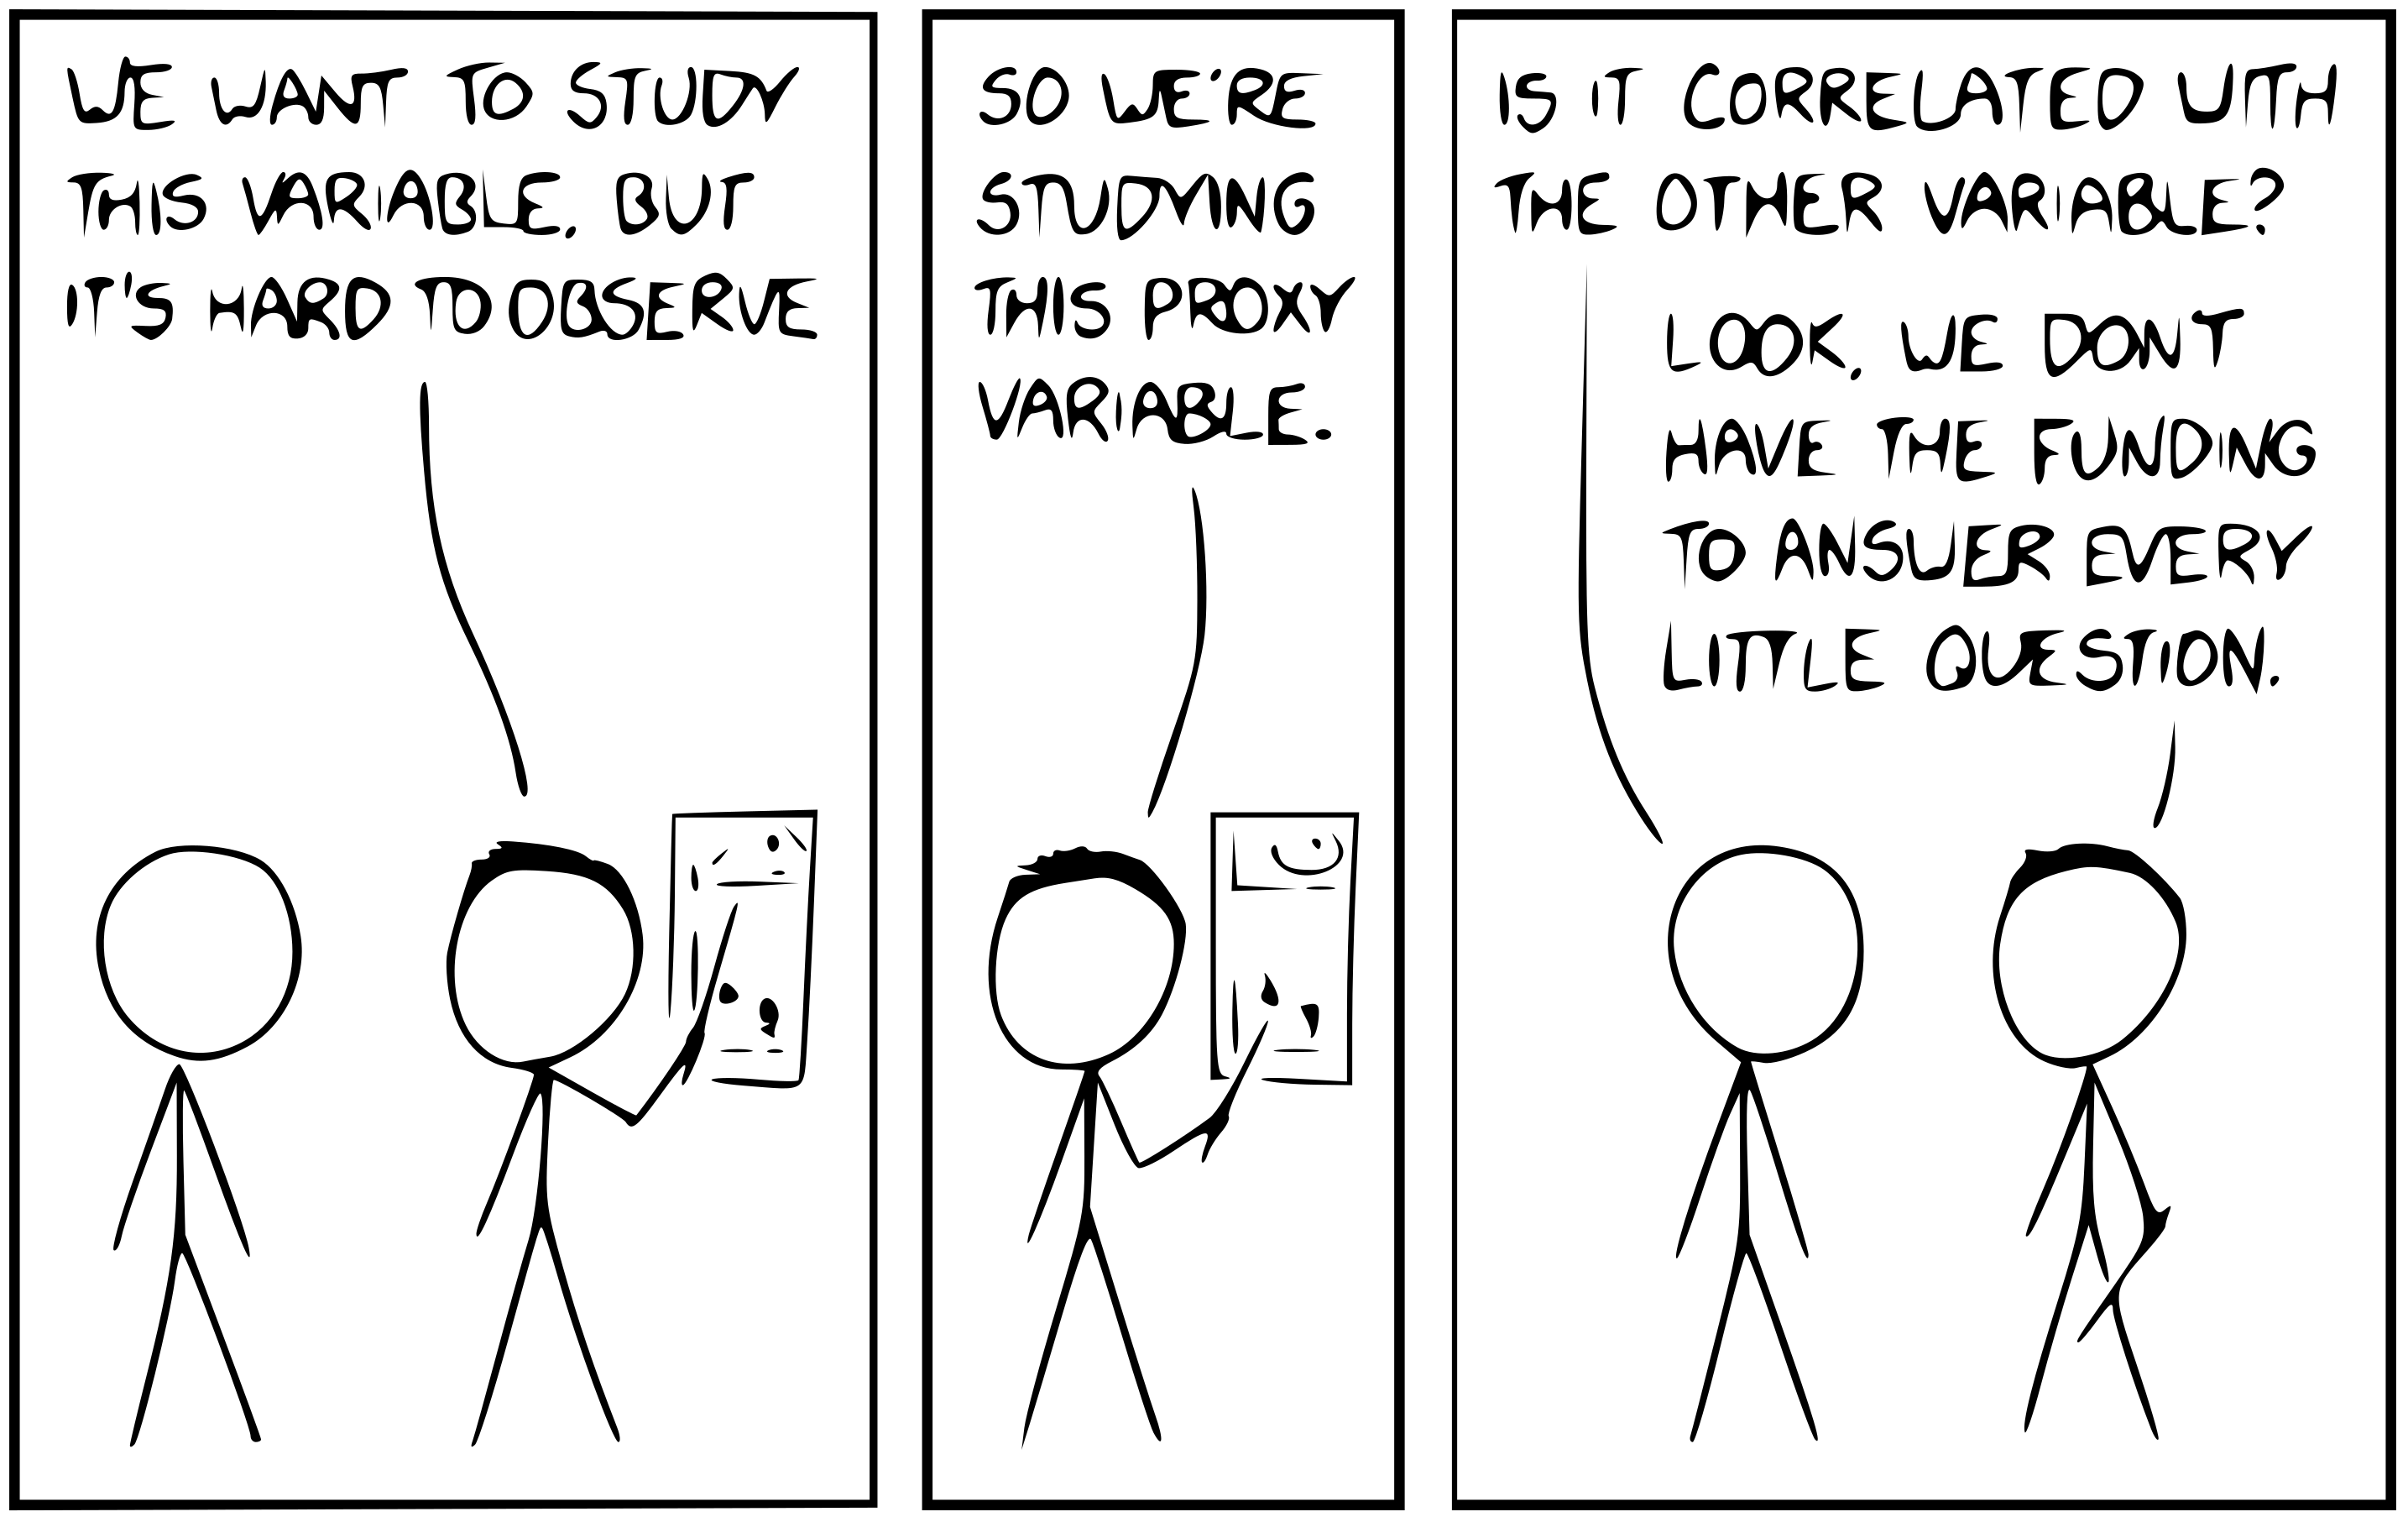
\includegraphics[width=\linewidth]{ch.discussion/imgs/xkcd.png}
    \caption{RNA-seq is a proxy for gene regulation and protein expression, but its relation to those remains poorly understood. \textbf{xkcd}. URL: https://xkcd.com/2652}
    \label{fig:xkcd}
\end{figure}

% \subsection{Stop blaming "the incentives"}

% incentives: https://www.talyarkoni.org/blog/2018/10/02/no-its-not-the-incentives-its-you/

\subsection{Self-correcting}

e.g. wild growth covid papers

papers keep on being cited after retraction or criticism. Number one paper of percentage of genome is functional gives highly criticized ENCODE paper.

highlight cancer microbiome paper: https://www.nature.com/articles/s41586-020-2095-1. And the negative result : https://www.biorxiv.org/content/10.1101/2023.07.28.550993v1.full.pdf

comparison of mouse vs human transcriptome: https://www.pnas.org/doi/full/10.1073/pnas.1413624111 and the re-analysis that they were wrong: https://f1000research.com/articles/4-121/v1

ENCODE claiming 80\% biochemical and criticism on it. When googling first result is ENCODE (I think)

Our golden standard is actual clinical trials! Our methods don't seem to work so well..?
https://www.ncbi.nlm.nih.gov/pmc/articles/PMC6409418/
https://journals.plos.org/plosmedicine/article?id=10.1371/journal.pmed.0020124

% Biology is messy, but that does not mean computational biology has to be.

\subsection{Universal gene regulatory networks}

It doesn't make sense to make GRNs between two specific cell types, or two developmental stages. There is a single set of instructions (DNA). So it should be possible to have a single universal GRN. (e.g. avocado).

Moreover, perhaps it is important to ask ourselves what is ultimately the goal of these GRNs? Do we care about having a map with all the arrows? Because the current correlation-based networks won't help us with differentiation networks. 